\cotefile{85}
\scanpage{86}
une \unsure{décomposition} en produit $\frac12$ direct
\[
L=G*\gamma\simeq G\underset{1/2}{\cdot}\unsure{E|\mathcal E}
\]
On va interpréter $E$ en notant qu'on a un hom (\unsure{inj|inj.})
\[
\gamma \overset{\rho}{\hookrightarrow} E
\]
et une op. de $G$ sur $E$, d'où pour $\sigma\in G$ un hom
\[
\gamma\overset{{}^{\sigma}\rho}{\unsure{\mathrel{\relbar}|\longrightarrow}}E\qquad
\deleted{\unsure{{}^{\sigma}\rho(x)={}^{\sigma}\rho(x)\,\rho}}
\inserted{{}^{\sigma}\rho=\sigma_E\circ\rho.}
\]
La famille des hom de groupes permet donc de définir un hom
\[
\underbrace{\gamma^{(*G)}}_{\text{puiss. libre}}\longrightarrow E
\]
\deleted{et une op. de}

D'ailleurs l'op. de $G$ sur l'ens d'indices $G$ permet de faire opérer $G$ sur la puiss. libre $\gamma^{(*G)}$, et \deleted{\unsure{par}} on voit que l'hom précédent est compatible aux op. de $G$. \deleted{En fait, on voit \unsure{trivialemt|tout de suite} que c'est un} \inserted{Donc on trouve}
\[
G\underset{1/2}{\cdot}\bigl(\gamma^{*G}\bigr)\longrightarrow L\simeq
G\underset{1/2}{\cdot}E
\]
On voit de suite que cet hom de groupes est un \uline{iso} (cf propriété universelle) donc
\[
\gamma^{(*G)}\xrightarrow{\sim}E\qquad \text{\uuline{iso}}
\]
% archive sheet number: 85
\scanpage{87}
% archive sheet number: 86
En prenant $G={\unsure{G|\mathfrak S|\mathcal S}}_3$, $\gamma=\widehat{\mathbb Z}^{\unsure{\times|*}}$ comme dessus, on trouve donc
\diagram{\begin{tikzcd}[ampersand replacement=\&,column sep=large,row sep=large]
G_3*\gamma \arrow[d, "{\substack{\text{via l'op. de }G_3\text{ sur }\unsure{\Pi|\Gamma|\Omega}\\ \text{et }\rho_{\varepsilon1.}}}" description] \&[-1em] \simeq \&[-1em] G_3\underset{1/2}{\cdot}\gamma^{(*G_3)}\\
\Omega \& \&
\end{tikzcd}}
% slanted
\margin{On peut prendre ici les \unsure{gr.} au sens profini \ldots}

Cet hom n'est pas injectif -- on a des relations, \deleted{\unsure{qui|pour}} \inserted{notamment l'une} exprimant la commutation des $\rho_{\varepsilon1.}$ et $\rho_{1\varepsilon'.}=\pi\rho_{\varepsilon.1}\pi^{-1}$ ($\pi=\pi_{01}$ transposition de $0$ et $1$) donc on va définir dans $\gamma^{(*G_3)}$ un \deleted{sous}groupe quotient inv. par $G_3$, en divisant par les relations exprimant
\[
\rho^{\pi}_{\deleted{\unsure{\varepsilon}}}\varepsilon\ \text{commute à}\ \rho^1(\varepsilon')\qquad
(\varepsilon,\varepsilon'\in\gamma)
\]
On trouve
\[
G_3\underset{1/2}{\cdot}\,\overset{\overset{\simeq}{\longrightarrow}}{\unsure{E|\mathcal E}}
(\gamma^2*\gamma^2*\gamma^2)=(\gamma^2)^{(*G_3/\unsure{\pi|2}}
\]
où $E$ est le produit libre \inserted{(profini)} des trois copies de $\gamma^2$, permutées transitivt entre elles par les op. de $G_3$, et un hom
\diagram{\begin{tikzcd}[ampersand replacement=\&,column sep=small]
G_3\underset{1/2}{\cdot}\deleted{\unsure{\gamma}}(\gamma\times\gamma)^{(*G_3/\pi_{01})}
 \arrow[r]\arrow[dr] \& \Omega^+ \arrow[d,dash] \&[-1em] \subset \&[-1em] \Omega \\
\& \widetilde{\Omega}^{+} \&[-1em] \subset \&[-1em] \widetilde{\Omega}\arrow[u,phantom,"\rotatebox{90}{$\subset$}" description]
\end{tikzcd}}
Il serait intéressant d'examiner les propriétés d'inj. et surjectivité de ces flèches, de $=$ que les variantes discrètes
\margin{$\gamma_0=\{\pm1\}$}
\diagram{\begin{tikzcd}[ampersand replacement=\&,column sep=small]
G_3\underset{1/2}{\cdot}(\gamma_0\times\gamma_0)^{(*G_3/\pi_{01})}
 \arrow[r]\arrow[dr] \& \Omega_0^+\arrow[d] \&[-1em] \subset \&[-1em] \Omega_0\arrow[d] \\
\& \widetilde{\Omega}_0^+ \&[-1em] \subset \&[-1em] \widetilde{\Omega}_0
\end{tikzcd}}
\scanpage{88}
Par définition $=$ de $\Omega^+$ etc, il est clair que les images sont les $\Omega^+$ etc (mais a-t-on $\Omega^+=\Omega$ etc ?) \margin{?} L'image de $\unsure{E|\mathcal E}$\inserted{$=(\gamma\unsure{*|\times}\gamma)^{(*{\unsure{G|\mathfrak S|\mathcal S}}_3/\pi_{01})}$} resp. $E_0$ est évidemment $|E|$ (resp. $|E|\unsure{.|{}_0}$) \ldots

On a un hom d'inclusion $\gamma_0\mathbin{-}\gamma$, définissant
\diagram{\begin{tikzcd}[ampersand replacement=\&,row sep=tiny]
(\gamma_0\times\gamma_0)^{*(G_3/\pi_{01})}\arrow[r] \&(\gamma*\gamma)^{(*G_3/\pi_{01})}\\
\rotatebox{90}{$=$}\&\rotatebox{90}{$=$}\\
E_0\&E
\end{tikzcd}}
et donnant lieu à diagramme comm.
\diagram{\begin{tikzcd}[ampersand replacement=\&,column sep=large]
G_3\underset{1/2}{\cdot} E_0\arrow[r,dash]\arrow[d] \& G_3\cdot E\arrow[d]\\
\Omega_0\arrow[r] \& \Omega.
\end{tikzcd}}

On a aussi, notant que
\diagram{\begin{tikzcd}[ampersand replacement=\&,column sep=small]
\gamma \&[-1em] = \&[-1em] \overset{\substack{\deleted{\unsure{\gamma}}\\\rotatebox{90}{$=$}}}{\widehat{\mathbb Z}^{*}}\arrow[r,dash,"{\deleted{\unsure{\sim}}}"] \&(\mathbb Z/6\mathbb Z)^*\arrow[r,"\sim"]\&(\mathbb Z/3\mathbb Z)^*\arrow[r,dash,"\sim"]\&\pm1\\
\gamma_0\arrow[u,hook] \&[-1em] = \&[-1em] \mathbb Z^*\arrow[u,hook]\arrow[urrr,bend right=16,"\sim"']\&\deleted{\unsure{\gamma_2|\chi_2}}\ \deleted{\unsure{\gamma_0=\mathbb Z^*|\chi_0=\mathbb Z^*}}\arrow[u]\&\&
\end{tikzcd}}
un hom $\gamma\longrightarrow\gamma_0$ inv. à g. de $\gamma_0\hookrightarrow\gamma$, d'où $E\longrightarrow E_0$ inv à g. de $E_0\mathbin{-}E$, d'où
\[
G_3\cdot E\mathbin{\text{---}}G_3\cdot E_0
\]
inv. à g. de \unsure{tt} à l'heure. D'autre part considérons
\[
\deleted{\unsure{\Omega}}\Pi(6)=\text{quotient de }\Pi\text{ par \deleted{la} \inserted{\unsure{(l'introduct de)|(l'adhérence de)}} relation }
\underset{\deleted{\unsure{h^6}}\ g^6=1\quad(g\in\Pi_0)}{\vphantom{\Pi}\strut}
\]
% archive sheet number: 87
\scanpage{89}
\deleted{\unsure{On|e}}et \unsure{a}
\[
\begin{aligned}
\Omega(6)&=\mathrm{Aut}(\Pi(6))\\
\widetilde{\Omega}(6)&=\mathrm{Aut}\,\mathrm{ext}(\Pi(6))
\end{aligned}
\]
de sorte qu'on a un hom \unsure{évident|induit|induits}
\diagram{\begin{tikzcd}[ampersand replacement=\&]
\Omega.\arrow[r]\arrow[d]\&\Omega(6)\arrow[d]\& \text{et un au \unsure{niv.} des}\\
\widetilde{\Omega}\arrow[r]\&\widetilde{\Omega}(6)\&
\end{tikzcd}}
Ceci dit, l'hom composé
\diagram{\begin{tikzcd}[ampersand replacement=\&,column sep=small]
{\unsure{G|\mathfrak S|\mathcal S}}_3\cdot(\gamma\times\gamma)^{(*G_3/\pi_{01})}\arrow[r,dash]\arrow[dr]\&\Omega\arrow[r,dash]\&\Omega(6)\\
\text{se factorise en}\&G_3\cdot(\gamma_0\times\gamma_0)^{(*G_3/\pi_{01})}\arrow[ur]\&
\end{tikzcd}}
i.e. les op. ``\unsure{él|èl|él.}'' au sens profini, ou au sens discret, deviennent les $=$, dès lors qu'on opère dans $\Pi(6)$ au lieu de $\Pi$. On peut dire que si $H$ est un gpe où tt él. est d'ordre divisant $6$ (p.ex. $H\simeq A_4$) alors l'op. de $G_3\underset{1/2}{\cdot}|\unsure{E|\mathcal E|\mathbb E}|\unsure{\simeq|\xrightarrow{\sim}}\Omega^+$ sur l'ens $\unsure{\mathscr T|\mathcal T}(H)$ ou $\mathrm{Sch}(H)$ se fait par l'intermédiaire de $G_3\underset{1/2}{\cdot}|E|_0\simeq\Omega_0^+$ -- donc aussi par l'intermédiaire de $G_3\underset{1/2}{\cdot}(\gamma_0\times\gamma_0)^{(*G_3/\pi_{01})}$.
% archive sheet number: 88
\scanpage{90}
Ce groupe est engendré par ${\unsure{G|\mathfrak S|\mathcal S}}_3$ et $6$ éléments $\rho_\sigma$ ($\sigma\in G_3$) \deleted{$\rho_\sigma=\sigma$} avec relations
\[
\begin{aligned}
\left\{\begin{aligned}
\rho_\sigma&=\sigma\rho_1\sigma^{-1}\quad\inserted{(\sigma\in G_3)}
  \quad[\text{donc }\rho_{\tau\sigma}=\tau\rho_\sigma\tau^{-1}\ \inserted{(\sigma,\tau\in G_3)}]\\
\rho_1^2&=1\qquad [\Rightarrow \rho_\sigma^2=1]\\
\rho_1\rho_\pi&=\rho_\pi\rho_1\qquad(\pi=\pi_{01}\ \text{transposition de }0,1)
\end{aligned}\right.\\
[\Rightarrow(\rho_\sigma\rho_{\sigma\pi}=\rho_{\sigma\pi}\rho_\sigma\qquad]
\end{aligned}
\]
Le groupe \deleted{\unsure{qui sera}} (des ``opérations'' élémentaires discrètes'') opère p.ex. sur l'ens des $72+24=96$ syst. de Schwartz \inserted{$\mathrm{Sch}(H)$} d'un groupe tétraédral $H(\simeq A_4)$, donc sur l'ens $\widetilde{\mathrm{Sch}}(H)$ formé de $8$ éléments $[(3,3,2)^+\ (3,3,2)^-$ et les transformés par $G_3^+$, $(3,3,3)^+$ et $(3,3,3)^-]$, donc sur l'ens à $4$ élts, des classes sous \deleted{Comme on a explicité \unsure{déj.}} $\widetilde H=\mathrm{Aut}(H)$ $(\simeq G_{\unsure{4|3}})$, formé de $(3,3,2)$ $(3,\deleted{\unsure{3}}2,3)$ $(2,3,3)$ et de $(3,3,3)$. Comme on a explicité l'action de $G_3$ sur ces ens, il \unsure{restera|resterait} à expliciter l'action de $\unsure{E|\mathcal E}_0$, ou ce qui revient dès lors au $=$, de $\rho_1$ i.e. $\rho_{-1,1.}$ L'exercice est immédiat en fonction de ce qui a été vu. \deleted{\unsure{pour}} Il serait intéressant d'expliciter les gpes quotients finis de $G_3\cdot E_0$ qui opèrent \uline{fidmt} sur les \unsure{$3/$ens|$3$ ens.} précédents \ldots
% archive sheet number: 89
\scanpage{91}
\uline{NB} De façon générale, s'intéressant aux gpes $H$ (finis) dans lesquels chaque él. est d'ordre \deleted{fini} divisant un entier $N$ fixé ($N=6$ pour le gpe tétraédral, $N=12$ pour celui ${\unsure{G|\mathfrak S|\mathcal S}}_4$ de l'octaèdre, $N=30$ pour celui $A_5$ de l'icosaèdre) on est amené à remplacer $\Pi$ par le quotient correspondant $\Pi(N)$, $\Omega$ par $\Omega(\deleted{\unsure{6}}N)=\mathrm{Aut}(\Pi(N))$, \deleted{et} $G_3\underset{1/2}{\cdot}|\unsure{E|\mathcal E|\mathbb E}|$ par $G_3\underset{1/2}{\cdot}|E|(N)$, quotient de \deleted{$G_3\underset{1/2}{\cdot}(\gamma(N)\times\gamma(N))$}
\[
\left\{\begin{aligned}
&G_3\underset{1/2}{\cdot}(\gamma(N)\times\unsure{\gamma|\sigma}(N))^{(*\deleted{\unsure{\gamma}}G_3/\pi_{01})}\\
&\text{où}\qquad\gamma(N)=(\mathbb Z/N\mathbb Z)^*
\end{aligned}\right.
\]
\[
\left[\,\gamma(N)\simeq
\left|\begin{aligned}
&\pm1 &&\text{pour }A_{\deleted{\unsure{5}}4}\\
&(\pm1)\times(\pm1)&&\text{pour }G_{\deleted{\unsure{5}}4}\\
&(\pm1)\times(\mathbb Z/4)&&\text{pour }A_5\\
&(\pm1)\times(\pm1)\times(\mathbb Z/4)&&\text{pour }G_5\qquad\text{etc.}
\end{aligned}\right.\right.
\]
% archive sheet number: 90
\scanpage{92}
\[
\begin{aligned}
\deleted{\rho}\unsure{\varepsilon|\xi}_1:\quad
 (\unsure{h|\ell}_0,h_1,\underset{\substack{\rotatebox{90}{$=$}\\h_1^{-1}h_0^{-1}}}{h_2})
 &\longmapsto (h_0^{-1},h_1,h_1^{-1}h_0=h_2h_0^2)\\
\deleted{\rho}\varepsilon_2:\quad(h_0,h_1,h_2)&\mathrel{\mapstochar\relbar}(h_0,h_1^{-1},h_1h_0^{-1}=h_1^2h_2)\\
\deleted{\rho}\varepsilon'_1:\quad(h_0,h_1,h_2)&\mathrel{\mapstochar\relbar}(h_{2}^{-1}h_1,h_1^{-1},h_2)=\\
\varepsilon'_2&\\
\deleted{\rho}\varepsilon''_1&\\
\deleted{\rho}\varepsilon''_2:\quad(h_0,h_1,h_2)&\longmapsto(h_0^{-1},h_0h_2^{-1},h_2^{\deleted{\unsure{+1|-1}}})
\end{aligned}
\]

\[
\begin{aligned}
\rho_1=\deleted{\rho}\varepsilon_1\deleted{\rho}\varepsilon''_2:\qquad
 h_0&\longmapsto h_0^{-1}\mathrel{\mapstochar\relbar}h_0\\
 h_1&\longmapsto h_0h_2^{-1}\longmapsto h_0^{-1}h_0^{-1}h_1=h_0^{-2}h_1\\
 h_2&\mathrel{\mapstochar\relbar}h_2\longmapsto h_1^{-1}h_0=h_2h_0^2\\
{\deleted{\rho}\varepsilon''_2}^{-1}\deleted{\rho}\varepsilon_1^{-1}:\qquad
 h_0&\mathrel{\mapstochar\relbar}\unsure{h^{-1}|h_0^{-1}|\ell_0^{-1}}\mathbin{\text{---}}h_0\\
 h_1&\longmapsto h_1\mathrel{\mapstochar\relbar}h_0h_2^{-1}=h_{\unsure{0}}^2h_1\\
 h_2&\mathrel{\mapstochar\relbar}h_1^{-1}h_0\longrightarrow h_2^{\deleted{\unsure{-1}}}h_0^{-1}h_0^{-1}=h_2h_0^{-2}
\end{aligned}
\]
\[
(\rho_1\rho''_2)^2\qquad\qquad\qquad x,
\]
\diagram{\begin{tikzcd}[ampersand replacement=\&,column sep=small,row sep=small]
\mathbb Z^3\arrow[r]\&\mathbb Z^3\arrow[r]\&\mathbb Z\\
\mathbb Z\arrow[u]\&V(\mathbb Z)\&
\end{tikzcd}}
\[
\begin{aligned}
(x_0\ x_1\ x_2)&\longrightarrow(-x_0,x_1,x_0-x_1)\\
 e_0\quad e_1\quad e_2&\\
 e_1-e_0,\ e_2-e_0&
\end{aligned}
\]
\figure{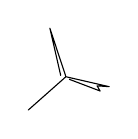
\begin{tikzpicture}[scale=.55,line cap=round,line join=round]
\draw (0,0)--(-.87,-.77) (0,0)--(-.37,1.12)--(-.12,.03) (0,0)--(1,-.23)--(.72,-.21)--(.79,-.33)--(.08,-.06);
\end{tikzpicture}}
\[
e_2=-e_0-e_1
\]
\diagram{\begin{tikzcd}[ampersand replacement=\&,column sep=small,row sep=tiny]
\deleted{\unsure{x+{}}}\mathbb Z\arrow[r]\&\mathbb Z^3\arrow[r,dash]\&\mathbb Z^3\\
\&e_{\unsure{1}}\arrow[r]\&e_{2}-e_3\\
\&e_2\arrow[r]\&{}
\end{tikzcd}}
\[
V^{\mathrm I}
\]
\[
\begin{aligned}
\deleted{(x,y,\unsure{z})}\quad\big[\, (e_0,e_1,e_2)&\longrightarrow(-e_0,e_1;e_0-e_1)\\
 (e_1,e_2,e_3)&\longrightarrow(e_0,-e_1\unsure{;|)}e_1-e_0)\\[2pt]
\big[\, (e_0,e_1,e_2)&\longmapsto(2e_1+e_0,-e_1\deleted{\unsure{)}};e_2\\
 (e_0,e_1,e_2)&\longmapsto\boxed{(-e_0-2e_1,\ e_1};-e_2)\\[2pt]
\big[\, [e_0,e_1,e_2)&\longmapsto\boxed{(e_0,\unsure{-2e_0-e_1}};-e_2)\\
 (e_0,e_1,e_2)&\longmapsto(-e_0,\unsure{2e_0+e_1},e_2)
\end{aligned}
\]
% archive sheet number: 91
\scanpage{93}
\figure{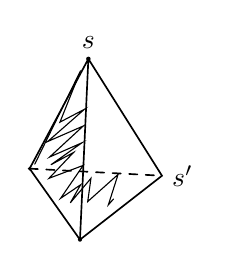
\begin{tikzpicture}[scale=.82,line width=.6pt,line cap=round]
\coordinate (t) at (0,2.1); \coordinate (b) at (-.13,-.7); \coordinate (l) at (-.91,.4); \coordinate (r) at (1.14,.29);
\draw (l)--(t)--(r)--(b)--cycle (t)--(b);
\draw[dashed] (l)--(r);
\draw[thin] (-.83,.47)--(-.12,1.92)--(-.44,1.12)--(-.06,1.32)--(-.63,.82)--(-.08,1.06)--(-.6,.58)--(-.1,.8)--(-.58,.46)--(-.23,.65)--(-.61,.25)--(-.08,.45)--(-.43,-.06)--(-.12,.15)--(-.28,-.13)--(.04,.25)--(-.01,-.11)--(.46,.31)--(.31,-.16)--(.39,-.07);
\fill (t) circle (.035) (b) circle (.032) (l) circle (.03);
\node[above] at (t) {$s$}; \node[right] at (r) {$s'$};
\end{tikzpicture}}
\[
\begin{aligned}
\beta\ \Sigma_r\qquad &(\rho_f,\rho_s,\rho_a) &&\text{\uline{$r$ direct}} &&(3,3,2)^+\\
&(\rho'_f,\rho'_s,\rho'_a) &&\text{\uline{$r$ inverse}} &&(3,3,2)^-\\
&(\rho_s,\rho_{s'},\rho_{s''}) &&(s,s',s'')\ \text{direct \unsure{autour sommet}} &&(3,3,3)^+\\
&(\rho'_s,\rho'_{s'},\rho'_{s''}) &&s,s',s''\ \text{inv. autour \unsure{som}} &&(3,3,3)^-\\
&\underset{\rho_f,\rho_{f'},\rho_{f''}}{\rotatebox{90}{$=$}}
\end{aligned}
\]
\[
\begin{aligned}
\deleted{(\rho_f^{-1},\rho_s,?}\qquad &(3,3,2)^+\longleftrightarrow(3,3,3)^+
  &&(\rho_{\unsure{s+|s|s'}}^{-1},\rho_{\unsure{f+|f|f'}}^{-1},\rho_{\unsure{a|.}}^{-1})\\
\rho_{s'}\qquad &(3,3,2)^-\longleftrightarrow(3,3,3)^-
  &&\underset{\rho_{f'}}{\rotatebox{90}{$=$}}\quad\rho_{s'}\quad
                \underset{\rho_a}{\rotatebox{90}{$=$}}\\
(\rho_f,\underset{\substack{\rotatebox{90}{$=$}\\\rho_{f'}}}{\rho_s^{-1}},?)\qquad
 &(3,3,2)^+\unsure{\mathbin{\text{---}}|\longleftrightarrow|\longleftarrow}(3,3,3)^-\\
 &(3,3,2)^-\longleftarrow(3,3,3)^+
\end{aligned}
\]
\[
\begin{aligned}
\Sigma_r &\qquad \Sigma'_r\\
{\unsure{G|\mathfrak S|\mathcal S}}_3^+\times R &\ \big\backslash\quad \deleted{\unsure{G_3^+}}\times R\\
72&\qquad24\\
\sigma\ \Sigma_r&\ \big|\quad \Sigma'_r\\
\underset{G_3^+}{\rotatebox{90}{$\in$}}\quad\underset{R}{\rotatebox{90}{$\in$}}&
\end{aligned}
\]
\[
\boxed{\sigma\cdot[r]\qquad\unsure{\{r'\}|\{r\}|\{r^{-1}\}}}
\]
\[
\tau\sigma[r]=\sigma^\tau\underline{\tau[r]}
\qquad \tau[r]=\left\{\vphantom{\Large A}\right.
\]
\[
G_3\cdot|\unsure{E|\mathcal E|\mathbb E}|_0\qquad\qquad
\unsure{h|\ell}_0\qquad h_0h_1h_0^{-1}\qquad h_0h_2h_0^{-1}
\]
\diagram{\begin{tikzcd}[ampersand replacement=\&,column sep=small,row sep=small]
\&\Pi_0\arrow[dl,dash]\arrow[r,phantom,"{\underset{\text{inv.}}{\subset}}" description]\&\Omega_0\arrow[d]\arrow[dl,dash]\&\\
{}\arrow[r,dash]\&{\mid}\,|E|_0\&G_3\&\mathbb E\mathrm{l}
\end{tikzcd}}
\[
\begin{aligned}
\rho_1\qquad &\rho_\sigma=\sigma\rho\sigma^{-1}
  &&\underset{-1\quad1}{\rule{1.6em}{.4pt}}\\
&\deleted{\rho_1\rho_\pi\quad\rho'_1\rho'_1}\\
&\overleftrightarrow{\rho_1\rho_2}\quad
  \overleftrightarrow{\rho'_1\rho'_2}\quad\overleftrightarrow{\rho''_1\rho''_2}
  &&\\[-1pt]
&\qquad\underset{\rho_\pi}{\rotatebox{90}{$=$}}
\end{aligned}
\]
\[
\deleted{\rho_1:\ h_0\mathbin{-}h_0^{\unsure{-1}}\quad h_1\longrightarrow}\qquad\rho_1
\]
\[
\begin{aligned}
&\tikz[baseline=(a.base)]{\node (a) {$\rho_1\rho''_2$}; \draw (a.center) ellipse (2.1em and .8em);}\\
&\tikz[baseline=(b.base)]{\node (b) {$\rho'_1\rho_2$}; \draw (b.center) ellipse (2.1em and .8em);}\\
&\tikz[baseline=(c.base)]{\node (c) {$\rho''_1\rho'_2$}; \draw (c.center) ellipse (2.1em and .8em);}
\end{aligned}
\]
\[
\begin{aligned}
x+y+z\ &=0\\
-x+y+&
\end{aligned}
\qquad
\begin{array}{cccccc}
(-1,\unsure{1|0},\unsure{-1|1})&(1,-1,-1)&(-1,-1,\unsure{1|0})&
(\unsure{1|0},-1,-1)&(0\ 0,-1)&(-1,0\ 0)\\[-1pt]
\multicolumn{6}{c}{\rule{.4pt}{.45em}\rule{.75\linewidth}{.4pt}\rule{.4pt}{.45em}}\\[-2pt]
\rho_1&\rho_2&\rho'_1&\rho'_2&\rho''_1&\rho''_2
\end{array}
\]
% archive sheet number: 92
\scanpage{94}
\[
\unsure{h|\ell}_0\ h_1\ h_2\longrightarrow
\begin{aligned}
&\deleted{\unsure{h_1h_0h_1^{-1}}h_0^{\unsure{1|0}}h_1}\\
&\deleted{h_0^{\unsure{\alpha_0}}h_1}
\end{aligned}
\]
\figure{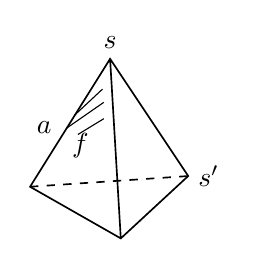
\begin{tikzpicture}[line width=.6pt,scale=.8]
\draw (-1.27,.02)--(0,2.05)--(1.24,.19)--(.17,-.8)--cycle (0,2.05)--(.17,-.8);
\draw[dashed] (-1.27,.02)--(1.24,.19);
\draw[thin] (-.57,1.15)--(-.12,1.57) (-.69,.95)--(-.1,1.36) (-.51,.85)--(-.1,1.1);
\node[above] at (0,2.05) {$s$}; \node[right] at (1.24,.19) {$s'$}; \node[left] at (-.77,.96) {$a$}; \node at (-.47,.67) {$f$};
\end{tikzpicture}}
\[
\begin{aligned}
 &(\overset{3}{\rho_f},\overset{3}{\rho_s},\overset{2}{\rho_a}) &&\unsure{3_3|\mathfrak S_3}\\
 &\rho_{s'}=\rho_f^{-1}\rho_s &&
 \begin{array}{l|l}
 \rho_{-1,1.}&(3,3,2)\longleftrightarrow(3,3,3)^-\\
 \rho_{1,-1.}&\deleted{\unsure{(3,3,2)}}\longleftarrow
 \end{array}\\
 &\rho_f\ \underset{\substack{\rotatebox{90}{$=$}\\\rho_{f'}}}{\rho_s^{-1}}
 &&\rho_{.\deleted{\unsure{-1}}-1,1}\\
 &\deleted{\rho_f}\quad\underset{\substack{\rotatebox{90}{$=$}\\\rho_{f'}}}{\rho_s^{-1}}\quad
 \underset{\substack{\rotatebox{90}{$=$}\\\rho_{a'}}}{\rho_a}
 &&\left\{\begin{array}{cc}(3,3,2)^+&\unsure{3.}\quad(3,3,2)^-\\
 (3,3,3)^+&(3,3,3)^-\end{array}\right.
\end{aligned}
\]
${\unsure{G|\mathfrak S|\mathcal S}}_3\cdot$\qquad opère sur \unsure{un|nos} ens à $8$ él.
\[
\begin{aligned}
\left.\begin{aligned}
 (3,3,2)^+ &\underset{\deleted{\rho_{-1,1,.}}}{\longleftrightarrow}(3,3,3)^+\\
 (3,3,2)^- &\longleftrightarrow(3,3,3)^-
\end{aligned}\right|&\ \rho_{-1,1,.}\\
\left.\begin{aligned}
 (3,3,2)\\ 3,3,2
\end{aligned}\right|&\ \rho_{1,-1,.}
\end{aligned}
\qquad
\tau_{01}\rho_{\alpha,1.}\tau_{01}^{-1}=\rho_{1,\alpha.}
\]
\[
\begin{aligned}
 &G_3*\mathbb Z/2\mathbb Z\\
 &\quad\unsure{\mathord{/}\ \rotatebox{90}{$\simeq$}|\wr\mathrel{\Vert}}\\
 &\deleted{\unsure{\mathbb Z}}\ G_3\cdot{\mathbb Z}_{/2\mathbb Z}^{(*G_3)}\\
 &\qquad\qquad\rho^\sigma(\varepsilon)
\end{aligned}
\]
\[
\begin{aligned}
&\unsure{\rho^{?}|\deleted{\rho_{\cdot}}}\qquad\\
&\rho_1^{\{01\}}((\varepsilon,1))\\
&\rho^{\{0,1\}}(\varepsilon,\varepsilon')\\
&\deleted{\rho_\sigma\quad\rho}
\end{aligned}
\qquad
\begin{aligned}
 &\rho(\varepsilon)\ \text{commute à}\ \rho^\sigma(\varepsilon),\\
 &\text{si }\sigma\text{ est une \inserted{de 2} transposition}\\
 &\deleted{\text{qui \unsure{change} }0.}\quad\inserted{\pi_{01},\pi_{02}}
\end{aligned}
\]
\[
\begin{aligned}
 &\varepsilon_\sigma\qquad(\sigma\in G_3)\\
 &\varepsilon_1=\rho^{\{01\}}\deleted{(\unsure{+1|1},1}(-1,1)=\rho_{-1,1.}\\
 &\pi\varepsilon_{\unsure{1|7}}\pi^{-1}=\rho_{1,-1.}\qquad\pi=\pi_{01}
\end{aligned}
\]
% archive sheet number: 93
\scanpage{95}
\margin{(3 p)}

Classes de ss-groupes de ${\unsure{G|\mathfrak S|\mathcal S}}_5$ et de ses sous-groupes.
% archive sheet number: 94
\scanpage{96}
les ss-groupes \deleted{$\unsure{G_3,\ Z_6,\ A_4}$}, $Z_3=A_3$, $Z_6$, ${\unsure{G|\mathfrak S|\mathcal S}}_2$, $G_3$, $D_3$, $\deleted{\unsure{G}}D_6$, correspondent $1$-$1$ aux triangles de $T$, $\boxed{\mathrm{Tr}(T)}$

les ss-groupes $Z_2$, $Z_4$, \deleted{$\unsure{D_2}$}, $\deleted{\unsure{D_4}}G_{22}$, $D_4$ \unsure{corresp|correspondent} $1$-$1$ aux carrés de $T$, $\boxed{\mathrm{Car}T}$

\noindent\rule{3.6em}{.4pt}\quad $D_2,A_4,G_4$\qquad\rule{5em}{.4pt}\quad pts de $T$\quad$\boxed{T}$

\noindent\rule{3.6em}{.4pt}\quad $Z_5,D_5$\qquad\rule{5em}{.4pt}\quad pent. de $T$\quad$\boxed{\mathrm{pent}(T)}$

\noindent\rule{3.6em}{.4pt}\quad $1,A_5,G_5$\quad sont invariants

\diagram{\begin{tikzcd}[ampersand replacement=\&,column sep=0pt,row sep=0pt]
{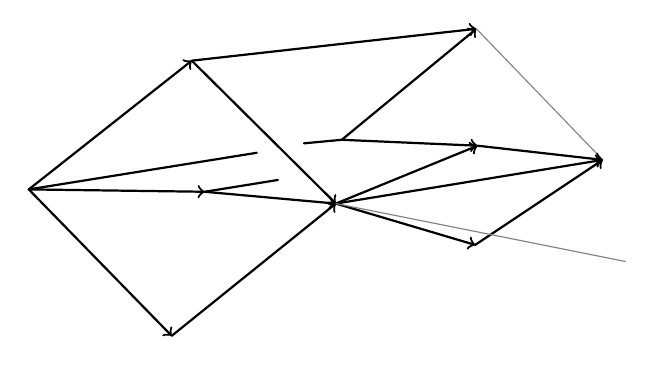
\begin{tikzpicture}[x=.015cm,y=-.015cm,line cap=round,line join=round,baseline=(current bounding box.center)]
\coordinate (l) at (17,109);
\coordinate (u) at (155,0);
\coordinate (b) at (138,233);
\coordinate (m) at (166,111);
\coordinate (r) at (277,121);
\coordinate (v) at (396,-27);
\coordinate (w) at (282,67);
\coordinate (c) at (397,72);
\coordinate (s) at (395,156);
\coordinate (z) at (503,84);
\draw[->,thick] (l)--(u);
\draw[->,thick] (u)--(r);
\draw[->,thick] (l)--(b);
\draw[->,thick] (b)--(r);
\draw[->,thick] (l)--(m);
\draw[->,thick] (m)--(r);
\draw[->,thick] (u)--(v);
\draw[->,thick] (w)--(v);
\draw[-,gray] (v)--(z);
\draw[->,thick] (w)--(c);
\draw[->,thick] (c)--(z);
\draw[->,thick] (r)--(c);
\draw[->,thick] (r)--(z);
\draw[->,thick] (r)--(s);
\draw[->,thick] (s)--(z);
\draw[thick] (l)--(210,78) (m)--(228,101) (w)--(250,70);
\draw[thin,gray] (r)--(522,170);
\end{tikzpicture}}
\end{tikzcd}}
Il y a $160$ ss-gpes $\ne 1,G_5$
\[
\begin{aligned}
\text{Nb de ss-gpes}\qquad &6\times10=60\\
+{}&4\times15=60\\
+{}&3\times5=15\\
+{}&2\times\deleted{\unsure{G_4}}12=24\\
+{}&\underline{3\times1=\phantom{2}3}\\
&\hphantom{3\times 1={}}162
\end{aligned}
\]
% crop-candidate: scan 96
\figure{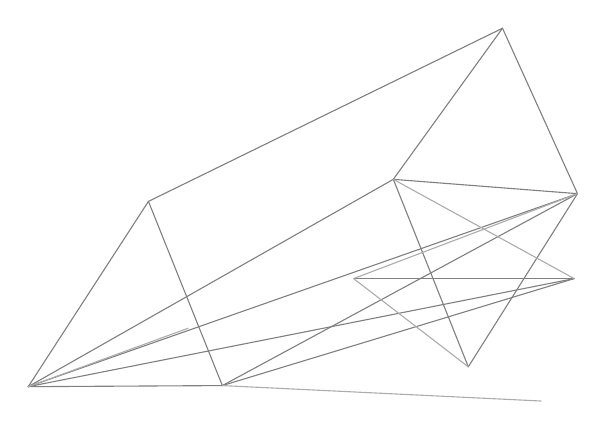
\begin{tikzpicture}[x=.014cm,y=-.014cm,line cap=round,line join=round,baseline=(current bounding box.center)]
\coordinate (l) at (0,325);
\coordinate (u) at (109,157);
\coordinate (r) at (176,324);
\coordinate (a) at (430,0);
\coordinate (b) at (331,137);
\coordinate (c) at (498,150);
\coordinate (d) at (399,307);
\coordinate (e) at (495,227);
\coordinate (f) at (295,227);
\draw[-,gray] (l)--(u);
\draw[-,gray] (u)--(r);
\draw[-,gray] (r)--(l);
\draw[-,gray] (u)--(a);
\draw[-,gray] (a)--(c);
\draw[-,gray] (c)--(b);
\draw[-,gray] (b)--(a);
\draw[-,gray] (b)--(d);
\draw[-,gray] (d)--(c);
\draw[-,gray] (l)--(b);
\draw[-,gray] (l)--(c);
\draw[-,gray] (r)--(c);
\draw[-,gray] (r)--(e);
\draw[-,gray] (e)--(f);
\draw[-,gray] (f)--(e);
\draw[-,gray] (l)--(e);
\draw[gray!65] (r)--(465,338) (f)--(d) (f)--(c) (b)--(e) (l)--(145,272);
\end{tikzpicture}}
\margin{\tikz[baseline=(n.base)]{\node[align=center] (n) {déterminer les\\ centralisateurs\\ d'éléments du\\ groupe $G_5$};\draw (n.north east) .. controls +(35:.3) and +(40:.5) .. (n.south east) .. controls +(-130:.6) and +(-70:.4) .. (n.south) .. controls +(145:.6) and +(-70:.6) .. (n.west) .. controls +(95:.5) and +(90:.3) .. (n.north east);}}
\diagram{\begin{tikzcd}[ampersand replacement=\&,column sep=0pt,row sep=0pt]
{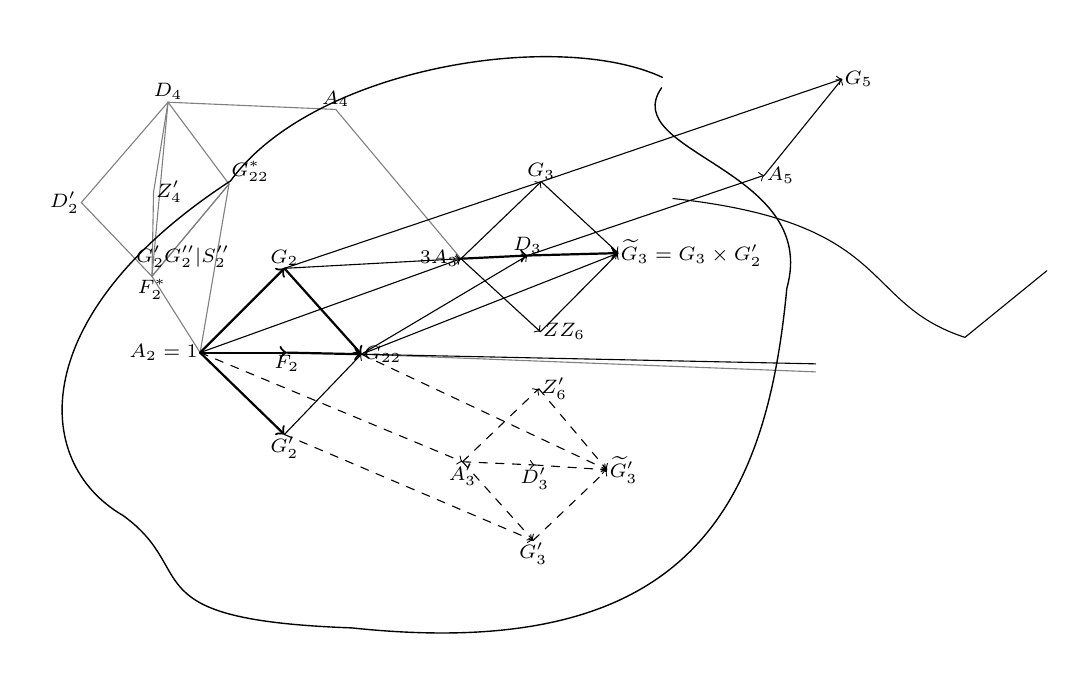
\begin{tikzpicture}[x=.0102cm,y=-.0102cm,line cap=round,line join=round,baseline=(current bounding box.center)]
\coordinate (D) at (165,788);
\coordinate (p) at (57,913);
\coordinate (z) at (147,900);
\coordinate (kk) at (145,1005);
\coordinate (sstar) at (241,890);
\coordinate (Al) at (374,797);
\coordinate (one) at (205,1100);
\coordinate (g) at (310,995);
\coordinate (f) at (313,1100);
\coordinate (gp) at (310,1202);
\coordinate (v) at (406,1102);
\coordinate (a) at (530,983);
\coordinate (h) at (630,887);
\coordinate (d) at (613,979);
\coordinate (zz) at (629,1074);
\coordinate (k) at (726,976);
\coordinate (ap) at (532,1236);
\coordinate (dp) at (622,1240);
\coordinate (zp) at (627,1145);
\coordinate (hp) at (620,1334);
\coordinate (kp) at (712,1246);
\coordinate (A) at (908,879);
\coordinate (G) at (1005,759);
\draw[-,gray] (D)--(p);
\draw[-,gray] (p)--(kk);
\draw[-,gray] (kk)--(D);
\draw[-,gray] (D)--(z);
\draw[-,gray] (z)--(kk);
\draw[-,gray] (D)--(sstar);
\draw[-,gray] (sstar)--(kk);
\draw[-,gray] (kk)--(one);
\draw[-,gray] (sstar)--(one);
\draw[-,gray] (D)--(Al);
\draw[-,gray] (kk)--(sstar);
\draw[-,gray] (Al)--(a);
\draw[->,thick] (one)--(g);
\draw[->,thick] (g)--(v);
\draw[->,thick] (one)--(f);
\draw[->,thick] (f)--(v);
\draw[->,thick] (one)--(gp);
\draw[->] (gp)--(v);
\draw[thin] (g)--(h);
\draw[->] (v)--(k);
\draw[->] (a)--(h);
\draw[->] (h)--(k);
\draw[->,thick] (a)--(d);
\draw[->,thick] (d)--(k);
\draw[->] (a)--(zz);
\draw[->] (zz)--(k);
\draw[->] (one)--(a);
\draw[->] (g)--(a);
\draw[->] (v)--(d);
\draw[->] (d)--(A);
\draw[->] (h)--(G);
\draw[->] (A)--(G);
\draw[dashed,->] (one)--(ap);
\draw[dashed,->] (gp)--(hp);
\draw[dashed,->] (v)--(kp);
\draw[dashed,->] (ap)--(hp);
\draw[dashed,->] (hp)--(kp);
\draw[dashed,->] (ap)--(dp);
\draw[dashed,->] (dp)--(kp);
\draw[dashed,->] (ap)--(zp);
\draw[dashed,->] (zp)--(kp);
\draw[gray] (v)--(972,1124);
\draw[thin] (v)--(972,1114);
\draw[line width=.5pt] (781,757) .. controls (650,696) and (345,745) .. (243,886) .. controls (-9,1050) and (-8,1235) .. (109,1303) .. controls (206,1373) and (115,1433) .. (394,1443) .. controls (810,1487) and (910,1297) .. (936,1020) .. controls (978,871) and (724,851) .. (780,770);
\draw[thin] (1158,1081) .. controls (1026,1038) and (1072,938) .. (794,908) (1158,1081)--(1260,998);
\node[anchor=south,inner sep=.7pt,font=\scriptsize] at (D) {$D_4$};
\node[anchor=east,inner sep=.7pt,font=\scriptsize] at (p) {$D'_2$};
\node[anchor=west,inner sep=.7pt,font=\scriptsize] at (z) {$Z'_4$};
\node[anchor=north,inner sep=.7pt,font=\scriptsize] at (kk) {$\mathbb F_2^*$};
\node[anchor=south west,inner sep=.7pt,font=\scriptsize] at (sstar) {$G_{22}^*$};
\node[anchor=south,inner sep=.7pt,font=\scriptsize] at (Al) {$A_4$};
\node[anchor=east,inner sep=.7pt,font=\scriptsize] at (one) {$A_2=1$};
\node[anchor=south,inner sep=.7pt,font=\scriptsize] at (g) {$G_2$};
\node[anchor=east,inner sep=.7pt,font=\scriptsize] at (245,981) {$\unsure{G'_2G''_2|\mathfrak S''_2}$};
\node[anchor=north,inner sep=.7pt,font=\scriptsize] at (f) {$F_2$};
\node[anchor=north,inner sep=.7pt,font=\scriptsize] at (gp) {$G'_2$};
\node[anchor=west,inner sep=.7pt,font=\scriptsize] at (v) {$G_{22}$};
\node[anchor=east,inner sep=.7pt,font=\scriptsize] at (a) {$\deleted{\unsure{3}}A_3$};
\node[anchor=south,inner sep=.7pt,font=\scriptsize] at (h) {$G_3$};
\node[anchor=south,inner sep=.7pt,font=\scriptsize] at (d) {$D_3$};
\node[anchor=west,inner sep=.7pt,font=\scriptsize] at (zz) {$\deleted{\unsure{Z}}Z_6$};
\node[anchor=west,inner sep=.7pt,font=\scriptsize] at (k) {$\widetilde G_3=G_3\times G'_2$};
\node[anchor=north,inner sep=.7pt,font=\scriptsize] at (ap) {$A'_3$};
\node[anchor=north,inner sep=.7pt,font=\scriptsize] at (dp) {$D'_3$};
\node[anchor=west,inner sep=.7pt,font=\scriptsize] at (zp) {$Z'_6$};
\node[anchor=north,inner sep=.7pt,font=\scriptsize] at (hp) {$G'_3$};
\node[anchor=west,inner sep=.7pt,font=\scriptsize] at (kp) {$\widetilde G'_3$};
\node[anchor=west,inner sep=.7pt,font=\scriptsize] at (A) {$A_5$};
\node[anchor=west,inner sep=.7pt,font=\scriptsize] at (G) {$G_5$};
\end{tikzpicture}}
\end{tikzcd}}
\[
\boxed{\begin{aligned} Z_2&\simeq G_2\\ D_2&\simeq G_{2,2}\\ D_3&\simeq G_3\end{aligned}}
\]
\figure{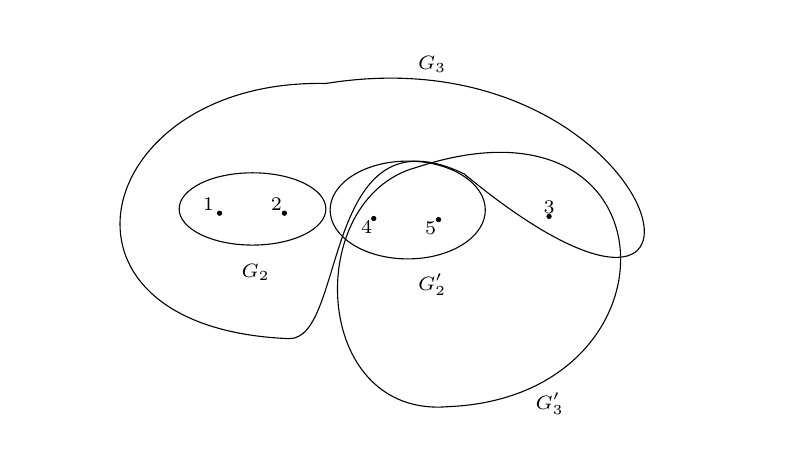
\begin{tikzpicture}[x=1.35cm,y=-1.35cm,line cap=round,line join=round,baseline=(current bounding box.center)]
\draw (1.5,1.1) .. controls (-.7,1.05) and (-1.3,3.4) .. (1.15,3.5) .. controls (1.7,3.52) and (1.45,1.3) .. (2.8,1.95) .. controls (5.65,4.3) and (4.7,.58) .. (1.5,1.1);
\draw (2.35,1.89) .. controls (1.28,2.18) and (1.36,4.25) .. (2.65,4.14) .. controls (4.9,4.05) and (4.82,1.07) .. (2.35,1.89);
\draw (.81,2.28) ellipse (.69 and .34) (2.27,2.29) ellipse (.73 and .46);
\foreach \x/\y in {.5/2.32,1.11/2.32,1.95/2.37,2.56/2.38,3.6/2.35}{\fill (\x,\y) circle (.025);}
\node[anchor=south east,inner sep=.7pt,font=\scriptsize] at (.47,2.32) {$1$};
\node[anchor=south east,inner sep=.7pt,font=\scriptsize] at (1.11,2.32) {$2$};
\node[anchor=north east,inner sep=.7pt,font=\scriptsize] at (1.96,2.37) {$4$};
\node[anchor=north east,inner sep=.7pt,font=\scriptsize] at (2.56,2.38) {$5$};
\node[anchor=south,inner sep=.7pt,font=\scriptsize] at (3.6,2.35) {$3$};
\node[anchor=south,inner sep=.7pt,font=\scriptsize] at (2.5,1.02) {$G_3$};
\node[anchor=north,inner sep=.7pt,font=\scriptsize] at (.84,2.78) {$G_2$};
\node[anchor=north,inner sep=.7pt,font=\scriptsize] at (2.5,2.87) {$G'_2$};
\node[anchor=north west,inner sep=.7pt,font=\scriptsize] at (3.45,3.99) {$G'_3$};
\end{tikzpicture}}
\[
\begin{aligned}
&\underline{1}\\
&\deleted{\unsure{G_2}}\quad\unsure{\rotatebox{90}{$=$}}\\
&Z_2\quad Z_3\quad Z_4\quad Z_5\quad Z_6\\
&D_2\quad D_3\quad D_4\quad D_5\\
&\underset{G_{2,2}}{\rotatebox{90}{$\simeq$}}\quad
 \underset{\deleted{\unsure{G_3}}}{\rotatebox{90}{$\simeq$}}\quad
 \deleted{\unsure{G_4,\ G_5}}\\
&\deleted{A_4,\ G_4,\ A_5,\ G_5}\\
&\deleted{\widetilde G_3=G_3\times}\quad A_4\quad A_5
\end{aligned}
\]
\diagram{\begin{tikzcd}[ampersand replacement=\&,column sep=0pt,row sep=0pt]
{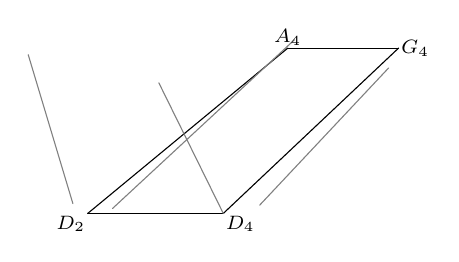
\begin{tikzpicture}[x=.021cm,y=-.021cm,line cap=round,line join=round,baseline=(current bounding box.center)]
\coordinate (D) at (0,100);
\coordinate (d) at (82,100);
\coordinate (a) at (121,0);
\coordinate (s) at (188,0);
\draw[thin] (D)--(d);
\draw[thin] (d)--(s);
\draw[thin] (s)--(a);
\draw[thin] (a)--(D);
\draw[gray] (15,97)--(125,-5) (104,95)--(182,12) (-9,94)--(-36,4) (d)--(43,21);
\node[anchor=north east,inner sep=.7pt,font=\scriptsize] at (D) {$D_2$};
\node[anchor=north west,inner sep=.7pt,font=\scriptsize] at (d) {$D_4$};
\node[anchor=south,inner sep=.7pt,font=\scriptsize] at (a) {$A_4$};
\node[anchor=west,inner sep=.7pt,font=\scriptsize] at (s) {$G_4$};
\end{tikzpicture}}
\end{tikzcd}}
\diagram{\begin{tikzcd}[ampersand replacement=\&,column sep=0pt,row sep=0pt]
{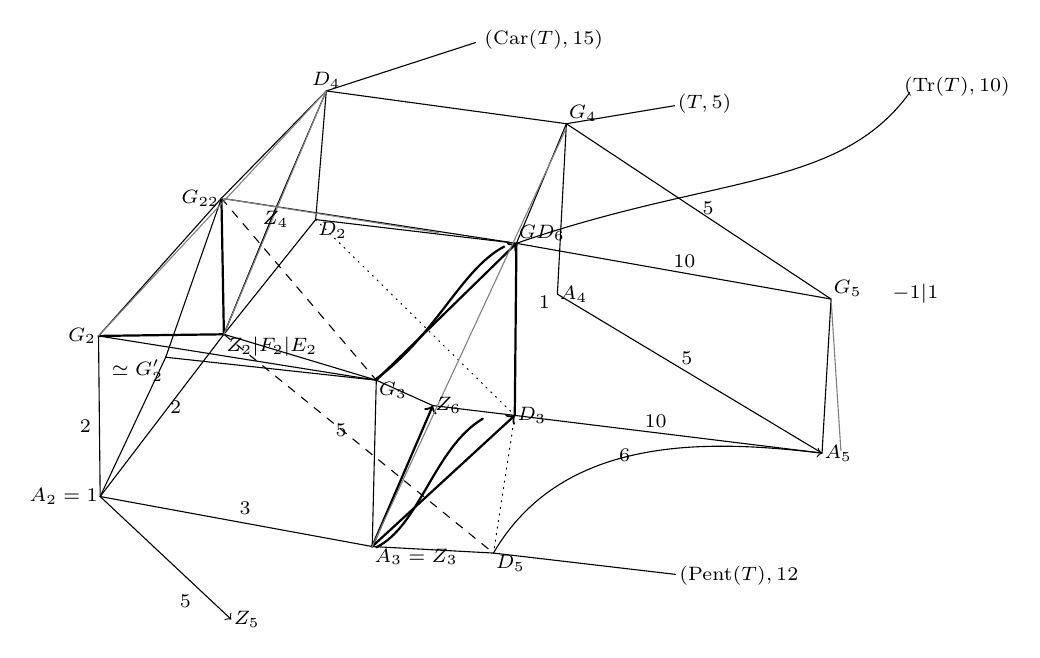
\begin{tikzpicture}[x=.0104cm,y=-.0104cm,line cap=round,line join=round,baseline=(current bounding box.center)]
\coordinate (D4) at (523,1699);
\coordinate (G4) at (816,1739);
\coordinate (V) at (395,1830);
\coordinate (Z4) at (461,1843);
\coordinate (D2) at (510,1856);
\coordinate (D6) at (755,1885);
\coordinate (G2) at (245,1998);
\coordinate (G2p) at (327,2024);
\coordinate (Z2) at (398,1996);
\coordinate (G3) at (584,2052);
\coordinate (Z6) at (653,2083);
\coordinate (D3) at (753,2095);
\coordinate (A4) at (805,1947);
\coordinate (G5) at (1139,1953);
\coordinate (A5) at (1128,2141);
\coordinate (A2) at (247,2194);
\coordinate (A3) at (579,2255);
\coordinate (D5) at (727,2263);
\coordinate (Z5) at (407,2344);
\draw[thin] (D4)--(G4);
\draw[thin] (D4)--(V);
\draw[thin] (V)--(G2);
\draw[thin] (D4)--(Z4);
\draw[thin] (Z4)--(Z2);
\draw[thin] (D4)--(D2);
\draw[thin] (D2)--(Z2);
\draw[thin] (V)--(G2p);
\draw[thin] (G2p)--(A2);
\draw[thin] (Z4)--(Z2);
\draw[-,thick] (V)--(Z2);
\draw[thin] (V)--(D6);
\draw[thin] (D2)--(D6);
\draw[dotted] (D2)--(D3);
\draw[thin] (G4)--(D6);
\draw[thin] (G4)--(A4);
\draw[thin] (G4)--(G5);
\draw[thin] (G5)--(A5);
\draw[thin] (D6)--(G5);
\draw[thin] (A4)--(A5);
\draw[thin] (D3)--(A5);
\draw[-,thick] (G2)--(Z2);
\draw[thin] (G2)--(G3);
\draw[thin] (G3)--(A3);
\draw[thin] (G2p)--(G3);
\draw[thin] (G2)--(A2);
\draw[thin] (A2)--(A3);
\draw[thin] (Z2)--(A2);
\draw[thin] (Z2)--(G3);
\draw[dashed] (Z2)--(D5);
\draw[dashed] (V)--(G3);
\draw[->,thick] (G3)--(D6);
\draw[-,thick] (D6)--(D3);
\draw[thin] (G3)--(Z6);
\draw[thin] (Z6)--(D3);
\draw[->,thick] (A3)--(Z6);
\draw[->,thick] (A3)--(D3);
\draw[thin] (A3)--(D5);
\draw[dotted] (D3)--(D5);
\draw[->] (A2)--(Z5);
\draw[->] (D5) .. controls (812,2117) and (991,2125) .. (A5);
\draw (D4)--(705,1640) (G4)--(948,1717) (D6) .. controls (997,1801) and (1149,1820) .. (1235,1701);
\draw (D5)--(949,2289);
\draw[thin,gray] (G2)--(D4) (V)--(660,1872) (A3)--(816,1744) (Z2)--(D4) (G5)--(1151,2138);
\draw[thick] (584,2256)..controls (637,2230) and (655,2134)..(714,2099) (583,2051)..controls(658,1996)and(688,1916)..(740,1889);
\node[anchor=south,inner sep=.7pt,font=\scriptsize] at (D4) {$\boxed{D_4}$};
\node[anchor=south west,inner sep=.7pt,font=\scriptsize] at (G4) {$\boxed{G_4}$};
\node[anchor=east,inner sep=.7pt,font=\scriptsize] at (V) {$G_{22}$};
\node[anchor=north,inner sep=.7pt,font=\scriptsize] at (Z4) {$Z_4$};
\node[anchor=north west,inner sep=.7pt,font=\scriptsize] at (D2) {$D_2$};
\node[anchor=south west,inner sep=.7pt,font=\scriptsize] at (D6) {$\boxed{\deleted{\unsure{G}}D_6}$};
\node[anchor=east,inner sep=.7pt,font=\scriptsize] at (G2) {$G_2$};
\node[anchor=north east,inner sep=.7pt,font=\scriptsize] at (G2p) {$\simeq G'_2$};
\node[anchor=north west,inner sep=.7pt,font=\scriptsize] at (Z2) {$\unsure{\mathbb Z_2|F_2|\mathbb E_2}$};
\node[anchor=north west,inner sep=.7pt,font=\scriptsize] at (G3) {$G_3$};
\node[anchor=west,inner sep=.7pt,font=\scriptsize] at (Z6) {$Z_6$};
\node[anchor=west,inner sep=.7pt,font=\scriptsize] at (D3) {$D_3$};
\node[anchor=west,inner sep=.7pt,font=\scriptsize] at (A4) {$A_4$};
\node[anchor=south west,inner sep=.7pt,font=\scriptsize] at (G5) {$\boxed{G_5}$};
\node[anchor=east,inner sep=.7pt,font=\scriptsize] at (1273,1947) {$\unsure{-1|1}$};
\node[anchor=west,inner sep=.7pt,font=\scriptsize] at (A5) {$A_5$};
\node[anchor=east,inner sep=.7pt,font=\scriptsize] at (A2) {$A_2=\boxed{1}$};
\node[anchor=north west,inner sep=.7pt,font=\scriptsize] at (A3) {$A_3=Z_3$};
\node[anchor=north west,inner sep=.7pt,font=\scriptsize] at (D5) {$\boxed{D_5}$};
\node[anchor=west,inner sep=.7pt,font=\scriptsize] at (Z5) {$Z_5$};
\node[anchor=west,inner sep=.7pt,font=\scriptsize] at (713,1636) {$(\mathrm{Car}(T),15)$};
\node[anchor=west,inner sep=.7pt,font=\scriptsize] at (949,1714) {$(T,5)$};
\node[anchor=west,inner sep=.7pt,font=\scriptsize] at (1225,1694) {$(\mathrm{Tr}(T),10)$};
\node[anchor=west,inner sep=.7pt,font=\scriptsize] at (951,2290) {$(\mathrm{Pent}(T),12$};
\node[anchor=center,inner sep=.7pt,font=\scriptsize] at (989,1842) {$5$};
\node[anchor=center,inner sep=.7pt,font=\scriptsize] at (960,1907) {$10$};
\node[anchor=center,inner sep=.7pt,font=\scriptsize] at (963,2025) {$5$};
\node[anchor=center,inner sep=.7pt,font=\scriptsize] at (925,2102) {$10$};
\node[anchor=north,inner sep=.7pt,font=\scriptsize] at (887,2133) {$6$};
\node[anchor=center,inner sep=.7pt,font=\scriptsize] at (789,1957) {$1$};
\node[anchor=center,inner sep=.7pt,font=\scriptsize] at (229,2108) {$2$};
\node[anchor=center,inner sep=.7pt,font=\scriptsize] at (339,2085) {$2$};
\node[anchor=center,inner sep=.7pt,font=\scriptsize] at (541,2113) {$5$};
\node[anchor=center,inner sep=.7pt,font=\scriptsize] at (424,2208) {$3$};
\node[anchor=center,inner sep=.7pt,font=\scriptsize] at (351,2322) {$5$};
\end{tikzpicture}}
\end{tikzcd}}
\[
\begin{array}{c|ccccc}
Z_1&\underline{Z_2}&\overset{A_3}{\underline{Z_3}}&\underline{Z_4}&\underline{Z_5}&\underline{Z_6}\\
\deleted{\unsure{D_1}}&\underline{D_2}&\underline{D_3}&\underline{D_4}&\underline{D_5}&\underline{D_6}\\
\deleted{\unsure{G_1}}&\underline{G_2}&\underline{G_3}&\underline{G_4}&\underline{G_5}&\\
\deleted{\unsure{A_1}}&\underline{1}=A_2&\underline{A_3}\mathrel{\rotatebox{45}{$=$}} Z_3&
 \underline{A_4},&\underline{A_5}&
\end{array}
\]
\[
\begin{aligned}
&G_{22}\\
&G''_2\times Z_2\quad \deleted{\unsure{\widetilde G_3=G_3\times|\mathfrak S_3\times}}\mathbb Z_2
\end{aligned}
\]
% archive sheet number: 95
\scanpage{97}
\figure{\begin{tikzpicture}[x=.0078cm,y=-.0078cm,line cap=round,line join=round,baseline=(current bounding box.center)]
\coordinate (apex) at (418,310);
\coordinate (west) at (251,557);
\coordinate (east) at (540,552);
\coordinate (low) at (365,797);
\coordinate (A) at (1078,1569);
\coordinate (B) at (940,1829);
\coordinate (C) at (1167,1831);
\coordinate (D) at (1368,1696);
\coordinate (E) at (1234,1948);
\coordinate (F) at (1458,1950);
\coordinate (G) at (1326,2206);
\coordinate (H) at (1034,2308);
\coordinate (J) at (947,2079);
\coordinate (K) at (1138,2096);
\coordinate (L) at (1046,1852);
\draw[thin] (apex)--(west) (265,556)..controls(365,553)and(444,539)..(529,548) (425,323)..controls(485,435)and(508,464)..(east) (252,560)--(362,790) (531,562)--(376,795);
\draw[gray] (343,781)--(285,625) (388,357)--(417,310)--(406,311)--(340,427) (410,345)--(495,516) (515,507)--(460,379) (395,775)--(541,562);
\draw[black!18,very thin] (1115,280)--(1237,379)--(1360,311)--(1488,410)--(1240,424)--(1115,457)--(1016,392) (1358,313)--(1183,291);
\draw[thin] (1020,383)--(1033,381) (1087,380)--(1095,380) (1109,378)--(1124,376) (1138,375)--(1168,373) (1144,384)--(1225,400);
\draw[black!20,very thin] (689,772)--(768,873) (769,873)--(1007,960)--(1143,1025) (1061,900)--(1185,981)--(1186,1004) (1010,1103)--(1153,982) (1388,1180)--(1459,1120);
\draw[thin] (1105,1027)--(1116,1020) (1125,1007)--(1141,993) (1185,991)--(1186,1004) (1021,1101)--(1031,1103) (1386,1181)--(1407,1181);
\draw[thick] (A)--(B);
\draw[thick] (B)--(C);
\draw[gray] (C)--(A);
\draw[thin] (A)--(D);
\draw[thin] (D)--(E);
\draw[thin] (E)--(B);
\draw[gray] (D)--(F);
\draw[gray] (F)--(E);
\draw[gray] (E)--(G);
\draw[thick] (F)--(G);
\draw[thin] (G)--(H);
\draw[thick] (H)--(J);
\draw[thick] (J)--(K);
\draw[gray] (K)--(H);
\draw[thick] (E)--(J);
\draw[thin] (J)--(L);
\draw[gray] (L)--(K);
\draw[gray!50,thin] (B)--(J) (L)--(H) (C)--(J) (D)--(G) (J)--(F);
\draw[thin] (905,1819)--(B)--(999,1821)--(1119,1805)--(C)--(1257,1866) (1315,1887)--(F)--(1370,2068) (956,1878)--(E) (1137,2098)--(1249,2056) (1035,2315)--(1324,2210);
\draw[gray] (924,1815)--(982,1683) (946,1815)--(1074,1573) (1093,1583)--(1154,1811) (939,2067)--(1223,1950) (943,2086)--(1023,2284) (1038,2293)--(1110,2136) (955,2080)--(1124,2090);
\end{tikzpicture}}
% crop-candidate: scan 97
% archive sheet number: 96
\scanpage{98}
\diagram{\begin{tikzcd}[ampersand replacement=\&,column sep=0pt,row sep=0pt]
{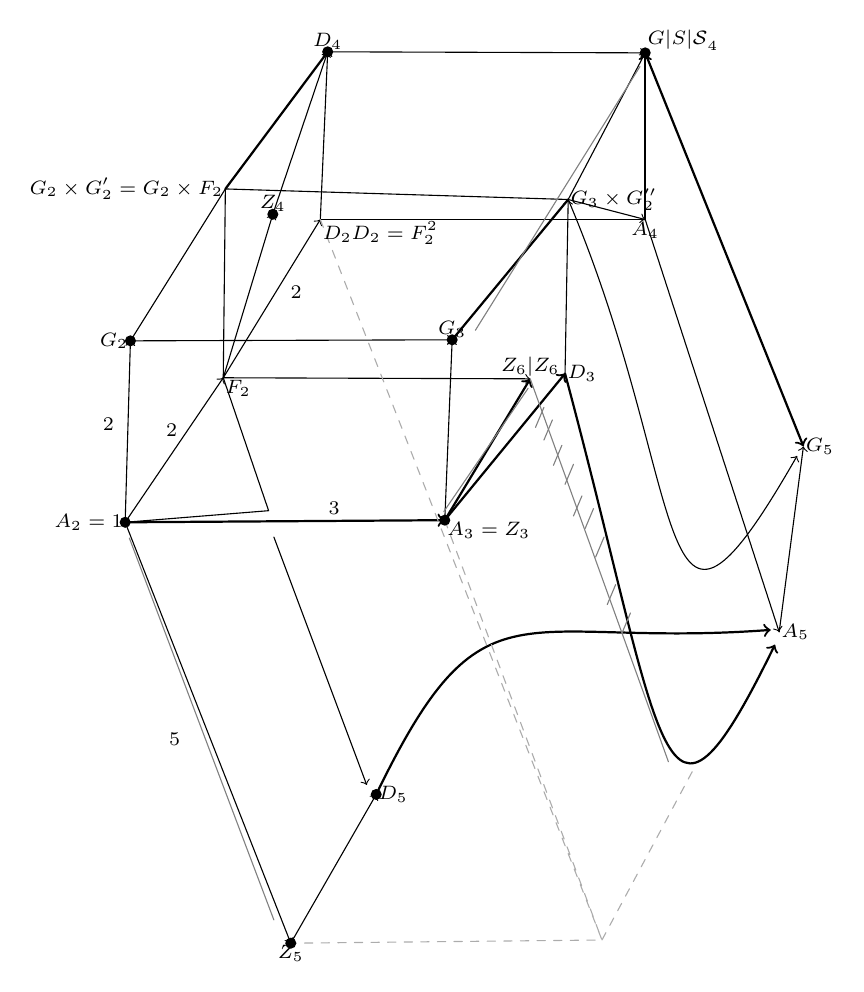
\begin{tikzpicture}[x=.0134cm,y=-.0134cm,line cap=round,line join=round,baseline=(current bounding box.center)]
\coordinate (D4) at (327,133);
\coordinate (G4) at (628,134);
\coordinate (V) at (230,263);
\coordinate (Z4) at (275,287);
\coordinate (D2) at (320,292);
\coordinate (D6) at (555,273);
\coordinate (A4) at (628,292);
\coordinate (G2) at (140,407);
\coordinate (F2) at (228,442);
\coordinate (G3) at (445,406);
\coordinate (Z6) at (519,443);
\coordinate (D3) at (552,438);
\coordinate (G5) at (778,507);
\coordinate (A2) at (135,579);
\coordinate (A3) at (438,577);
\coordinate (A5) at (755,683);
\coordinate (D5) at (373,837);
\coordinate (Z5) at (292,978);
\draw[->] (D4)--(G4);
\draw[-,thick] (V)--(D4);
\draw[->] (Z4)--(D4);
\draw[->] (D2)--(D4);
\draw[thin] (V)--(D6);
\draw[thin] (D2)--(A4);
\draw[->] (D6)--(A4);
\draw[->,thick] (A4)--(G4);
\draw[->,thick] (G4)--(G5);
\draw[thin] (G2)--(V);
\draw[->] (G2)--(G3);
\draw[thin] (V)--(F2);
\draw[->] (F2)--(Z4);
\draw[->] (F2)--(D2);
\draw[-,thick] (G3)--(D6);
\draw[->] (D6)--(G4);
\draw[->] (A3)--(G3);
\draw[->] (A2)--(G2);
\draw[->] (A2)--(F2);
\draw[->,thick] (A2)--(A3);
\draw[->] (F2)--(Z6);
\draw[->,thick] (A3)--(Z6);
\draw[->,thick] (A3)--(D3);
\draw[->] (D3)--(D6);
\draw[->] (A5)--(G5);
\draw[->] (A4)--(A5);
\draw[->] (A2)--(Z5);
\draw[->] (Z5)--(D5);
\draw[->] (276,593)--(364,828);
\draw (F2)--(271,568)--(A2);
\draw[->,thick] (D5) .. controls (475,626) and (506,699) .. (747,681);
\draw[->,thick] (D3) .. controls (648,796) and (642,918) .. (751,695);
\draw[->] (D6) .. controls (673,551) and (633,759) .. (772,516);
\draw[gray!65,dashed] (D2)--(587,975)--(Z5) (A3)--(587,975)--(676,809);
\draw[gray] (Z6)--(650,806) (139,594)--(276,956) (467,397)--(623,147) (437,569)--(517,452);
\foreach \a/\b in {4/0,12/4,21/12,32/18,40/28,51/32,61/41,72/56,86/65}{\draw[gray,thin] (528+\a,470+3*\b)--(520+\a,489+3*\b);}
\foreach \i in {A2,A3,G3,G2,Z4,D4,G4,D5,Z5}{\fill (\i) circle (2pt);}
\node[anchor=south,inner sep=.7pt,font=\scriptsize] at (D4) {$D_4$};
\node[anchor=south west,inner sep=.7pt,font=\scriptsize] at (G4) {${\unsure{G|\mathfrak S|\mathcal S}}_4$};
\node[anchor=east,inner sep=.7pt,font=\scriptsize] at (V) {$G_2\times G'_2=G_2\times\mathbb F_2$};
\node[anchor=south,inner sep=.7pt,font=\scriptsize] at (Z4) {$Z_4$};
\node[anchor=north west,inner sep=.7pt,font=\scriptsize] at (D2) {$\deleted{\unsure{D_2}}D_2=F_2^2$};
\node[anchor=west,inner sep=.7pt,font=\scriptsize] at (D6) {$G_3\times G''_2$};
\node[anchor=north,inner sep=.7pt,font=\scriptsize] at (A4) {$A_4$};
\node[anchor=east,inner sep=.7pt,font=\scriptsize] at (G2) {$G_2$};
\node[anchor=north west,inner sep=.7pt,font=\scriptsize] at (F2) {$F_2$};
\node[anchor=south,inner sep=.7pt,font=\scriptsize] at (G3) {$G_3$};
\node[anchor=south,inner sep=.7pt,font=\scriptsize] at (Z6) {$\deleted{\unsure{Z_6|\mathbb Z_6}}$};
\node[anchor=west,inner sep=.7pt,font=\scriptsize] at (D3) {$D_3$};
\node[anchor=west,inner sep=.7pt,font=\scriptsize] at (G5) {$G_5$};
\node[anchor=east,inner sep=.7pt,font=\scriptsize] at (A2) {$A_2=1$};
\node[anchor=north west,inner sep=.7pt,font=\scriptsize] at (A3) {$A_3=Z_3$};
\node[anchor=west,inner sep=.7pt,font=\scriptsize] at (A5) {$A_5$};
\node[anchor=west,inner sep=.7pt,font=\scriptsize] at (D5) {$D_5$};
\node[anchor=north,inner sep=.7pt,font=\scriptsize] at (Z5) {$Z_5$};
\node[anchor=center,inner sep=.7pt,font=\scriptsize] at (119,486) {$2$};
\node[anchor=center,inner sep=.7pt,font=\scriptsize] at (179,492) {$2$};
\node[anchor=center,inner sep=.7pt,font=\scriptsize] at (297,361) {$2$};
\node[anchor=center,inner sep=.7pt,font=\scriptsize] at (333,566) {$3$};
\node[anchor=center,inner sep=.7pt,font=\scriptsize] at (182,785) {$5$};
\end{tikzpicture}}
\end{tikzcd}}
les \deleted{\unsure{17}}18 \inserted{classes de} sous-groupes de $G_5$

\margin{\tikz[baseline=(q.base)]{\node[align=center] (q) {dont\\ 9 abéliens}; \draw (q.center) ellipse (3em and 1.8em);}}
\[
\begin{aligned}
[9]\ &\text{classes de ss-gpes de }A_5\\
11\ &\text{classes de ss-gpes de }G_4\\
5\ &\text{classes de ss-gpes de }A_4\\
4\ &\text{classes de ss gpes de }G_3\\
7\ &\text{classes de ss-gpes de }D_4\\
10\ &\rule{4.8em}{.5pt}\quad\widetilde G_3\\[-3pt]
&\quad\text{\uuline{\hspace{2.0em}}}
\end{aligned}
\]
\unsure{1}
\diagram{\begin{tikzcd}[ampersand replacement=\&,column sep=0pt,row sep=0pt]
{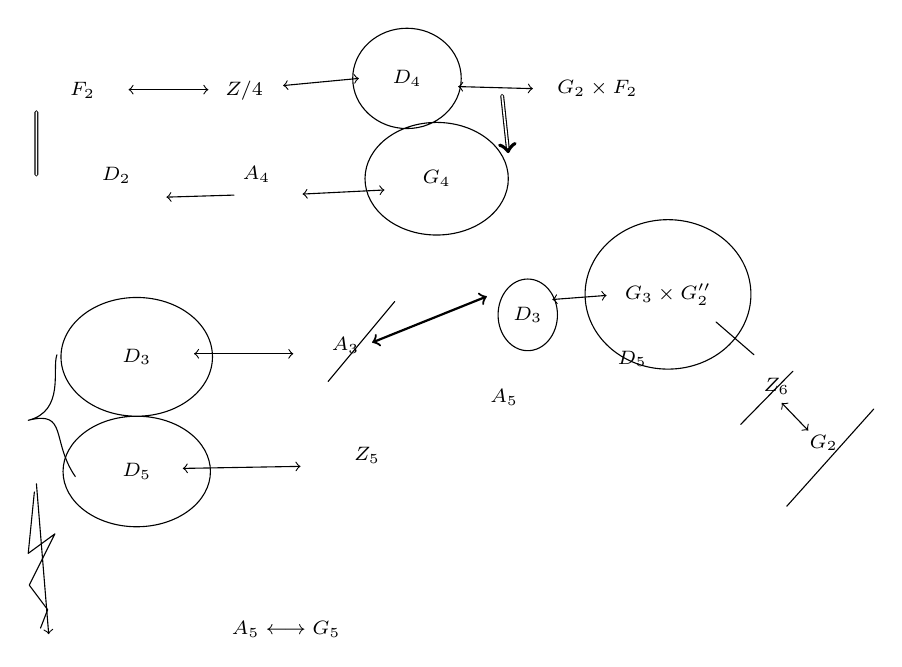
\begin{tikzpicture}[x=.013cm,y=-.013cm,line cap=round,line join=round,baseline=(current bounding box.center)]
\coordinate (f) at (95,1268);
\coordinate (z) at (253,1268);
\coordinate (d) at (412,1256);
\coordinate (v) at (598,1266);
\coordinate (p) at (128,1351);
\coordinate (a) at (265,1350);
\coordinate (s) at (441,1354);
\coordinate (D) at (148,1528);
\coordinate (A) at (352,1517);
\coordinate (Dprime) at (530,1487);
\coordinate (vprime) at (667,1467);
\coordinate (z6) at (773,1557);
\coordinate (g2) at (819,1612);
\coordinate (d5) at (148,1640);
\coordinate (z5) at (373,1624);
\draw[<->] (140,1267)--(218,1267);
\draw[<->] (291,1263)--(365,1256);
\draw[<->] (462,1264)--(535,1266);
\draw[->,double] (50,1289)--(50,1350) (505,1273)--(511,1329);
\draw[<-] (177,1372)--(243,1370);
\draw[<->] (310,1369)--(390,1365);
\draw (d) ellipse (53 and 49) (s) ellipse (70 and 55);
\draw[<->] (204,1525)--(301,1525);
\draw[<->,thick] (378,1514)--(490,1469);
\draw[<->] (554,1472)--(607,1468);
\draw[<->] (714,1494)--(751,1526) (778,1573)--(804,1600);
\draw[<->] (193,1637)--(308,1635);
\draw (D) ellipse (74 and 58) (d5) ellipse (72 and 54) (Dprime) ellipse (29 and 35) (vprime) ellipse (81 and 73);
\draw[thin] (335,1552)--(400,1474) (738,1594)--(789,1542) (783,1674)--(868,1579);
\draw (70,1526)..controls(65,1540)and(78,1581)..(42,1590)..controls(81,1580)and(64,1610)..(88,1645);
\draw[->] (50,1652)--(62,1799);
\draw[thin] (48,1660)--(42,1720)--(68,1701)--(43,1751)--(61,1775)--(54,1793);
\node[anchor=center,inner sep=.7pt,font=\scriptsize] at (f) {$F_2$};
\node[anchor=center,inner sep=.7pt,font=\scriptsize] at (z) {$\mathbb Z/4$};
\node[anchor=center,inner sep=.7pt,font=\scriptsize] at (d) {$D_4$};
\node[anchor=center,inner sep=.7pt,font=\scriptsize] at (v) {$G_2\times F_2$};
\node[anchor=center,inner sep=.7pt,font=\scriptsize] at (p) {$D_2$};
\node[anchor=center,inner sep=.7pt,font=\scriptsize] at (a) {$A_4$};
\node[anchor=center,inner sep=.7pt,font=\scriptsize] at (s) {$G_4$};
\node[anchor=center,inner sep=.7pt,font=\scriptsize] at (D) {$D_3$};
\node[anchor=center,inner sep=.7pt,font=\scriptsize] at (A) {$A_3$};
\node[anchor=center,inner sep=.7pt,font=\scriptsize] at (Dprime) {$D_3$};
\node[anchor=center,inner sep=.7pt,font=\scriptsize] at (vprime) {$G_3\times G''_2$};
\node[anchor=center,inner sep=.7pt,font=\scriptsize] at (z6) {$Z_6$};
\node[anchor=center,inner sep=.7pt,font=\scriptsize] at (g2) {$G_2$};
\node[anchor=center,inner sep=.7pt,font=\scriptsize] at (d5) {$D_5$};
\node[anchor=center,inner sep=.7pt,font=\scriptsize] at (z5) {$Z_5$};
\node[anchor=center,inner sep=.7pt,font=\scriptsize] at (507,1568) {$\deleted{\unsure{A_5}}$};
\node[anchor=center,inner sep=.7pt,font=\scriptsize] at (632,1530) {$\deleted{\unsure{D_5}}$};
\node[anchor=center,inner sep=.7pt,font=\scriptsize] at (294,1794) {$\deleted{\unsure{A_5\longleftrightarrow G_5}}$};
\end{tikzpicture}}
\end{tikzcd}}
\[
\left\{\begin{aligned}
F_2&=\mathfrak z(D_4)=\mathfrak z(D_4,G_4)\\
D_4&=N(F_2\unsure{,|;}G_4)\\
F_2&=2\cdot Z_4={}_2(Z_4)\\
D_4&=N(Z_4,G_4)\\
Z_4&=\text{gpe engendré par \unsure{l'un des|n'importe les|n'importe}}\\
 &\quad\text{\unsure{quels|quelconque|quel} des 2 \unsure{élts|élt|él.} d'ordre}\\
 &\quad 4\ \text{de }D_4
\end{aligned}\right.
\]
\[
\begin{aligned}
G_{\unsure{4|5}}&=N(D_2^{\unsure{2|*}},G_5)\\
D_2^{\unsure{2}}\!&=\text{seul sous-gpe invariant}\\
 &\quad\text{de }G_4\text{ d'indice }6
\end{aligned}
\]
\figure{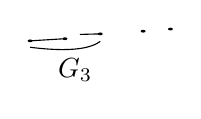
\begin{tikzpicture}[scale=.68]
\foreach \x/\y in {0/0,.65/.04,1.31/.13,2.11/.18,2.62/.22}{\fill (\x,\y) ellipse (.046 and .026);}
\draw (0,0)--(.65,.04) (.93,.12)--(1.31,.13);
\draw (0,-.12)..controls(.8,-.22)and(1.15,-.13)..(1.31,-.01);
\node[below] at (.84,-.14) {$G_3$};
\end{tikzpicture}}
\diagram{\begin{tikzcd}[ampersand replacement=\&]
G_{3}\arrow[d,dash]\\ A_{\unsure{2|6|3}}
\end{tikzcd}}
\diagram{\begin{tikzcd}[ampersand replacement=\&]
G_2\arrow[r,dash]\arrow[d,dash]\&G_3\arrow[r,dash]\arrow[d,dash]\&
G^{\unsure{1|'}}_{\unsure{3|2}}\times G'_{\unsure{3|2}}\arrow[d,dash]\\
{}\arrow[r,dash]\&A_3\arrow[r,dash]\&D_3
\end{tikzcd}}
% archive sheet number: 97
